%=================
\chapter{Planning}
%=================
This chapter explains the administrative part of the project. The project plan 
is presented in \autoref{sec:plan:project}. How the project is organized is 
covered in \autoref{sec:plan:org}, the quality assurance is described in 
\autoref{sec:plan:qa}, and how we are supposed to handle possible risk can be 
found in \autoref{sec:plan:risk}.

%---------------------
\section{Project Plan}
%---------------------
\label{sec:plan:project}
The project plan includes the specified plan on which tool we are using in this project, measurement of project effects, limitations and the concrete project work plan.

\subsection{Measurement of Project Effects}
%------------------------------------------
Automatic generation of \Gls{lua} \glspl{script} from \Gls{c} \gls{header} files would bring considerable resource savings in the customer's usual work process.
When the customer needs to know the contents of \gls{ipc} messages that include \Gls{c} \glspl{struct}, the use of our utility will save them time, and therefore financial resources.

The biggest impact on savings will be caused by enabling filtering of the messages by specific attributes in the \Gls{c} \gls{struct} in \Gls{wireshark}. Once this is made possible, searching for a specific \gls{struct} or \gls{member} will become easier.

Before creating the utility, \Gls{c} \glspl{struct} were investigated in two ways. The first, manual method, meant counting individual bytes of the \gls{binary} file that includes data in \Gls{c} \glspl{struct}. This was possible only for small-sized messages. For bigger messages, this method was inapplicable, as a message can consist of several thousands bytes. The second method consisted of manually writing a \gls{dissector} in \Gls{lua} for the specific \Gls{c} \gls{header}. Also, this method could not be used for more complex \Gls{c} \glspl{struct}, i.e. those using \glspl{nested struct}. At the start of this project there had been written around 10 \Gls{lua} \glspl{script} manually.

According to the customer, they had approximately 3000 \Gls{c} \glspl{struct} in their code base at the beginning of the project.
To debug all these structs, 3000 \glspl{dissector} needs to be written. Time spent writing a \gls{dissector} for a message manually depends on the \gls{struct}’s complexity. For simple \glspl{struct}, this takes around 15 minutes. It took about one hour for the most complicated \glspl{dissector} that the customer had developed so far.

If one hour is the average time for creating a \gls{dissector} for one message, our utility will be able to save around 3000 hours of work, not considering further changes to their code base. Due to everyday workload of the customer’s development team, this amount of time could never be used to accomplish such a task.

None of the methods mentioned above are capable of processing messages with \Gls{c} \glspl{struct} that are big and complex, making it difficult to estimate time savings in these cases.

In some cases, a representative of Thales Norway AS has to physically move to a customer’s site to solve a problem.
With the delivered solution, this can sometimes be avoided, since the customer can use Wireshark with the dissectors, and then send the capture files to Thales. This means that the problem in some cases can be solved in-house. Savings in this case are not only time-based, as this will also directly cut the transportation costs, as well as being an environmental benefit. It is also possible it will increase the satisfaction for the client.

\subsection{Limitations}
%-----------------------
As in all other projects, the project members had to deal with various limitations and constraints given either by the customer or personal limitations stemming from things such as lack of experience or conflicts with other personal responsibilities. The limitations as identified at the beginning of the project are listed below. 

\subsubsection{Technical Limitations}
\begin{description}
	\item[\Gls{c} \gls{preprocessor}] To fulfill all the requirements we might need to
		either modify an existing \gls{preprocessor} or write our own, which can be
		a highly time consuming process.
	\item[Platforms] Some of the platforms that are required for the utility are not
		available to the project team.
\end{description}

\subsubsection{Non-technical Limitations}
\begin{description}
	\item[Experience] No team members have experience with \Gls{lua}-\glspl{script},
		running a project with a larger team, or have planned a project before.
	\item[Time] The project team has a limited time of 13 weeks with a project
		deadline that cannot be changed. Also, the team consists of seven members
		that have different schedules so finding a time when everyone is
		available for a meeting might be difficult. These limitations might
		lead to considerable delays in the project progress.
	\item[Language] In this project the team will have to write and speak in
		English, which is a second language for all team members. This may
		lead to misunderstandings and will negatively affect the time it
		takes to write the report.
\end{description}

\subsection{Tool Selection}
%--------------------------
To support collaboration and project management the team has considered and
selected the listed tools for use in this project.

\subsubsection{Git \& Github}
\begin{wrapfigure}{r}{3.5cm}
	\vspace{-20pt}
	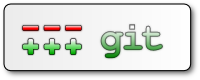
\includegraphics[width=3.5cm]{./planning/img/git_logo}
	\vspace{-20pt}
\end{wrapfigure}
The team selected Git as the \gls{version control system}, with git \gls{repository}
hosting provided by Github\footnote{\url{http://github.com/}}.

\begin{wrapfigure}{r}{3cm}
	\vspace{-20pt}
	
\includegraphics[width=3cm]{./planning/img/github_logo}
	\vspace{-20pt}
\end{wrapfigure}
We had experience with \Gls{cvs}, \Gls{svn}, Git and Mercurial, and although everyone 
knew \Gls{svn} and only two knew Git, we selected Git for this project.
The main reason we didn't choose \Gls{svn} was because of its lack of hosting capabilities,
and the other reason was that, unlike Git and Mercurial, \Gls{svn}	 does not have any of the
advantageous features of a modern \gls{version control system} like \glspl{branch} and a \gls{distributed
repository model}.

We evaluated free hosting sites of \glspl{version control system}, which could also 
provide us with other collaborative features that we wanted. Github, 
Bitbucket\footnote{\url{http://bitbucket.org/}} and
SourceForge\footnote{\url{http://sourceforge.net/}} all provided wiki and
issue tracker in addition to free \gls{version control system} hosting. We eliminated 
SourceForge because their focus is divided between software users and 
developers, while the other two sites are fully focused on developers. The 
two remaining sites provides almost identical features, where one focuses on 
Git and the other on Mercurial.

Github with Git \gls{version control system} was selected because more team members 
had experience with Git than Mercurial. Since we use different platforms,
we will also use different git clients, but for Windows most of the team has
selected tortoisegit.

\subsubsection{Skype}
\begin{wrapfigure}{r}{3cm}
	\vspace{-20pt}
	
\includegraphics[width=3cm]{./planning/img/skype_logo}
	\vspace{-20pt}
\end{wrapfigure}
Skype\footnote{\url{http://www.skype.com}} is an application which allows the
user to make video and voice chats over the Internet, including conference
calls and chatting. The team used Skype to communicate and collaborate when
we were not physically present at the same location at the same time.

\subsubsection{Google Docs}
\begin{wrapfigure}{r}{2cm}
	\vspace{-20pt}
	
\includegraphics[width=2cm]{./planning/img/google_docs_logo}
	\vspace{-20pt}
\end{wrapfigure}
Google Docs\footnote{\url{http://docs.google.com/}} is a free web site offering
functionality for creating documents, spreadsheets and presentations.
The benefits of using Google Docs are that it is easy to share documents with other users, and
it is possible to collaborate in real-time. For this project we used Google Docs
to collaborate on document drafts, and to share documents within the team and
with the team's advisor.

\subsubsection{\LaTeX}
\LaTeX \,is a document \gls{markup language} used to
create reports, articles and books. It was chosen by the team for its 
high quality typesetting which produces professional looking documents, and 
because it is suitable for larger scientific reports.\cite{NotSoShorGuideToLatex} 
Writing documents in \LaTeX \ is very different from writing them in, for example,
Microsoft Word, as most of the visual presentation is handled by the \LaTeX \ system 
and not by the user itself. Because the writer does not have to spend time
thinking about how the document looks, he can focus entirely on the content.
\LaTeX \,also provides automatic numbering of chapters and sections,
automatic generation of table of contents, cross-referencing and bibliography
management. Since \LaTeX \,files are plain text files they are suitable for versioning 
with a \gls{version control system} like Git. We will use \LaTeX \,to write the final project 
report, and we have created a few templates for test plans and minutes.

\subsubsection{Mailing List}
\begin{wrapfigure}{r}{4cm}
	\vspace{-20pt}
	
\includegraphics[width=4cm]{./planning/img/ntnu_logo}
	\vspace{-20pt}
\end{wrapfigure}
For asynchronous communication the team used an electronic mailing list
provided by \Gls{idi}, \Gls{ntnu}.

\subsubsection{Google Calendar}
\begin{wrapfigure}{r}{3cm}
	\vspace{-20pt}
	
\includegraphics[width=3cm]{./planning/img/google_calendar_logo}
	\vspace{-20pt}
\end{wrapfigure}
Since all team members have Google accounts, we created a team calendar
in Google Calendar\footnote{\url{http://calendar.google.com/}}
to help schedule and keep track of meetings. A single calendar that all
members can include in their own prevents misunderstandings and duplication
of work.

\subsubsection{text2pcap}
Since the customer could not provide us with capture files, 
we had to create them ourselves.  The capture files are important for testing
the generated \Gls{lua}-\glspl{script}. In this project text2pcap\footnote{\url{http://www.wireshark.org/docs/man-pages/text2pcap.html}} 
was used to generate capture files from ASCII\footnote{\url{http://www.asciitable.com/}}
\glspl{hex dump}.  The text2pcap tool is included with \Gls{wireshark}. 
The input to the tool is an ASCII \gls{hex dump} as a text-file, and the output will
be a \gls{pcap-file}.

\subsubsection{Hex Editor}
The team used a hex editor to create input for text2pcap. To make it
easier to write ASCII \glspl{hex dump}, it was deemed necessary to write them in a hex editor.
HxD\footnote{\url{http://mh-nexus.de/en/hxd/}} was the recommended hex editor
for this project, as it is free and has all of the necessary functionality.

\subsubsection{Violet}
\begin{wrapfigure}{r}{3cm}
	\vspace{-20pt}
	
\includegraphics[width=3cm]{./planning/img/violet_logo}
	\vspace{-20pt}
\end{wrapfigure}
Violet\footnote{\url{http://violet.sourceforge.net/}} is a free
and easy to use modeling software for making \Gls{uml}-diagrams.
It is also a cross platform solution, which means that all team members can use
the same application. If we had to use different \Gls{uml} applications there could be a problem
editing the diagrams due to incompatible file formats.
The architectural and design team used Violet to create diagrams
to illustrate the workings of the utility. As very advanced diagrams were not needed for
this project, Violet seemed like a fitting tool.

\subsection{Schedule of Results}
%-------------------------------
This project had two deliveries,a pre-delivery and a final delivery.
The milestones and sprints are listed below.

\subsubsection{Milestones}
\begin{tabular}{l l}
	30. August & Project start \\
	6. October & Pre-delivery of project report \\
	24. November & Final delivery of project report \\
	24. November & Presentation and project demo \\
\end{tabular}

\subsubsection{Sprints}
\begin{tabular}{l l}
	Sprint 1 & 14. September - 27. September \\
	Sprint 2 & 5. October - 18. October \\
	Sprint 3 & 19. October - 1. November  \\
	Sprint 4 & 2. November - 15. November \\
\end{tabular}

\subsection{Concrete Project Work Plan}
%--------------------------------------
The first two weeks of the project was used on planning and pre study.
The project was divided into four sprints that each lasted for two weeks.
The first sprint had an estimated length of 200 person-hours, while the last three
sprints had an estimate of 250 person-hours. The last one and a half weeks were used to finish
the final report and prepare for the presentation. \autoref{tab:wbs} shows the
work breakdown structure, and the project timeline is in \autoref{fig:gantt}.

\begin{table}[!htb] \footnotesize \center
\caption{Work Breakdown Structure\label{tab:wbs}}
\begin{tabular}{l l l c c}
	\toprule
	& & & \multicolumn{2}{c}{Effort} \\
	\cmidrule(r){4-5}
	Task & From date & To date & Estimated & Actual  \\
	\midrule
	Misc & 30.08.2011 & 24.11.2011 & 825 & 855  \\
	\midrule
	Project Management & 30.08.2011 & 24.11.2011 & 275 & 454 \\
	Lectures & 02.09.2011 & 18.10.2011 & 100 & 100 \\
	Self Study & 30.08.2011 & 04.10.2011 & 100 & 71 \\
	Planning & 05.09.2011 & 12.09.2011 & 150 & 122 \\
	Pre-study & 05.09.2011 & 12.09.2011 & 100 & 49 \\
	Requirement Specification & 05.09.2011 & 12.09.2011 & 100 & 59 \\
	\midrule
	Sprint 1 & 14.09.2011 & 27.09.2011 & 200 & 157 \\
	\midrule
	Sprint 1 Planning & 14.09.2011 & 14.09.2011 & 30 & 29 \\
	Sprint 1 Work & 15.09.2011 & 26.09.2011 & 150 & 98 \\
	Sprint 1 Review & 27.09.2011 & 27.09.2011 & 20 & 30 \\
	\midrule
	Sprint 2 & 05.10.2011 & 18.10.2011 & 250 & 260 \\
	\midrule
	Sprint 2 Planning & 05.10.2011 & 05.10.2011 & 30 & 36 \\
	Sprint 2 Work & 06.10.2011 & 17.10.2011 & 200 & 206 \\
	Sprint 2 Review & 18.10.2011 & 18.10.2011 & 20 & 18 \\
	\midrule
	Sprint 3 & 19.10.2011 & 01.11.2011 & 300 & 296 \\
	\midrule
	Sprint 3 Planning & 19.10.2011 & 19.10.2011 & 30 & 48 \\
	Sprint 3 Work & 20.10.2011 & 31.10.2011 & 250 & 234 \\
	Sprint 3 Review & 01.11.2011 & 01.11.2011 & 20 & 14 \\
	\midrule
	Sprint 4 & 02.11.2011 & 15.11.2011 & 300 & 311 \\
	\midrule
	Sprint 4 Planning & 02.11.2011 & 02.11.2011 & 30 & 34 \\
	Sprint 4 Work & 03.11.2011 & 14.11.2011 & 250 & 263 \\
	Sprint 4 Review & 15.11.2011 & 15.11.2011 & 20 & 14 \\
	\midrule
	Report \& Presentation & 30.08.2011 & 24.11.2011 & 400 & 452 \\
	\midrule
	Write Report & 20.08.2011 & 24.11.2011 & 325 & 388 \\
	Presentation & 22.11.2011 & 24.11.2011 & 75 & 64 \\
	\midrule
	Total & 30.08.2011 & 24.11.2011 & 2275 & 2331 \\
	\bottomrule
\end{tabular}
\end{table}

\begin{figure}[!htb]
	\noindent\makebox[\textwidth]{%
	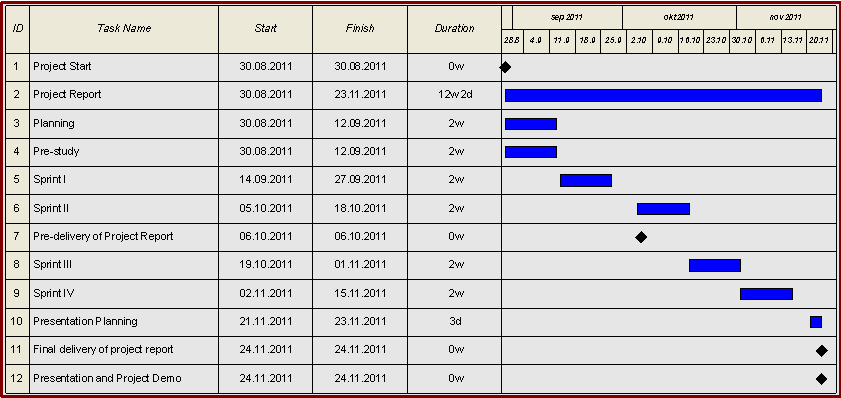
\includegraphics[scale=0.48]{./planning/img/gantt}}
	\caption{Gantt Diagram\label{fig:gantt}}
\end{figure}


%-----------------------------
\section{Project Organization}
%-----------------------------
\label{sec:plan:org}
This section describes how the team was organized, which roles the developers were divided into and the partners of the project.

\subsection{Project Organization}
%--------------------------------
Our project organization had a flat structure, and the organization chart can be seen in figure \ref{fig:orgchart}. The roles listed in the organization chart are described in table \ref{tab:roles}.

\begin{figure}[htb]
	\noindent\makebox[\textwidth]{%
	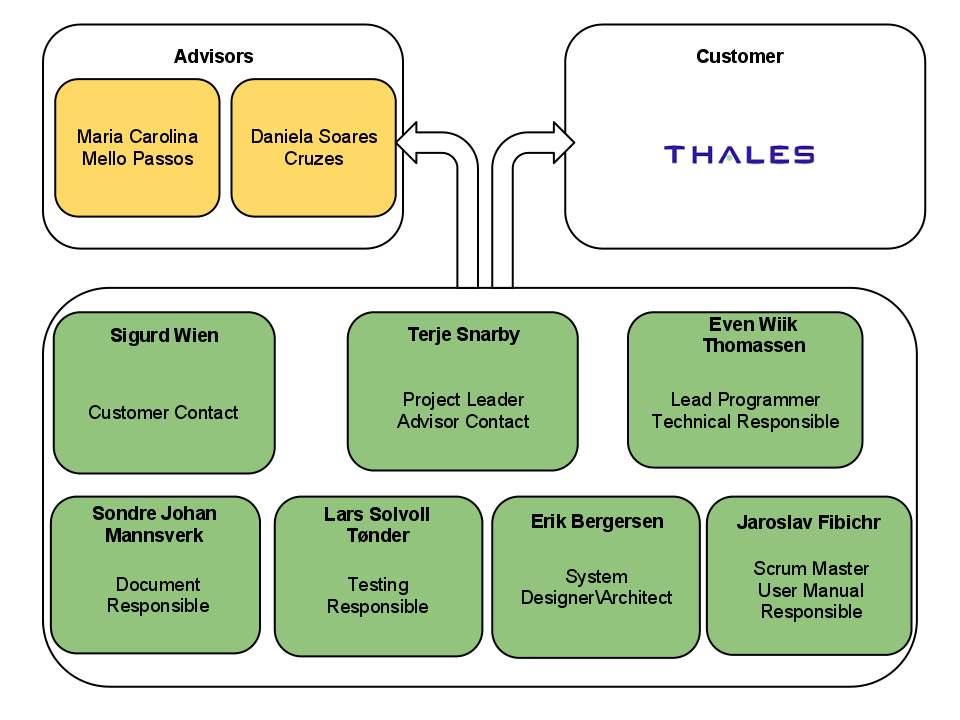
\includegraphics[scale=0.45]{./planning/img/organization}}
	\caption{Project Organization\label{fig:orgchart}}
\end{figure}

\begin{table}[!htb] \footnotesize \center
\caption{Project Roles\label{tab:roles}}
\noindent\makebox[\textwidth]{%
\begin{tabularx}{\textwidth}{l X}
	\toprule
	Role name & Main responsibilities  \\
	\midrule
	Project manager & Responsible for having an overview of the project, delegating tasks and resolving conflicts. \\ 
	Advisor contact & Responsible for distributing information between the team and the advisor. \\
	Organizer & Responsible for setting up and informing the team about the meeting schedule. \\ 
	Document master & Responsible for document quality and quantity. \\ 
	System architect & The lead designer of the system. \\ 
	Lead programmer & Makes sure everyone follows the agreed code standards, and ensures the quality of the code. \\ 
	Customer contact & Responsible for distributing information between the team and the customer. \\ 
	Technically responsible & Finds suitable technical solutions and makes sure that the essential tools are operative. \\ 
	Technology evangelist & Brings in ideas about new technologies and tools. \\ 
	Scrum master & Responsible for \Gls{scrum} meetings. \\ 
	Lead tester & Responsible for test coverage, both unit and end to end, and to ensure the quality of those tests. \\ 
	Secretary & Takes note from each meetings and stores it in the cloud. Responsible for preparing minutes for advisor/customer. \\
	\bottomrule
\end{tabularx}}
\end{table}

\subsection{Partners}
%--------------------
This subsection lists the partners of this project. The customer of this
project is Thales Norway AS, which is located at Lerkendal Stadium,
Strindveien 1, 7030 Trondheim. The customer contacts are listed in
\autoref{tab:plan:customer}. The development team consist of seven student
from \Gls{ntnu}, and is listed in \autoref{tab:plan:devs}. The team is assigned two
advisors from the Department of Computer and Information Science at \Gls{ntnu},
listed in \autoref{tab:plan:advisors}. 

\begin{table}[!htb] \footnotesize \center
\caption{Customers\label{tab:plan:customer}}
\begin{tabular}{l l l}
	\toprule
	Name & Mobile & E-mail \\ 
	\midrule
	Christian Tellefsen & 959 98 765 & christian.telefsen@thalesgroup.com \\ 
	Stig Bjørlykke & 982 29 806 & stig.bjorlykke@thalesgroup.com \\ 
	\bottomrule
\end{tabular}
\end{table}

\begin{table}[!htb] \footnotesize \center
\caption{Developers\label{tab:plan:devs}}
\begin{tabular}{l l l}
	\toprule
	Name & Mobile & E-mail  \\ 
	\midrule
	Terje Snarby & 915 27 390 & snarby@stud.ntnu.no \\ 
	Even Wiik Thomassen & 991 61 929 & evenwiik@stud.ntnu.no \\ 
	Sondre Johan Mannsverk & 948 15 506 & sondrejo@stud.ntnu.no \\ 
	Erik Bergersen & 917 48 305 & eribe@stud.ntnu.no \\ 
	Lars Solvoll Tønder & 976 00 317 & larssot@stud.ntnu.no \\ 
	Sigrud Wien & 472 54 625 & sigurdw@stud.ntnu.no \\ 
	Jaroslav Fibichr & 451 26 314 & jaroslaf@stud.ntnu.no \\ 
	\bottomrule
\end{tabular}
\end{table}

\begin{table}[!htb] \footnotesize \center
\caption{Advisors\label{tab:plan:advisors}}
\begin{tabular}{l l l}
	\toprule
	Name & Mobile & E-mail \\ 
	\midrule
	Daniela Soares Cruzes & 942 49 891 & dcruzes@idi.ntnu.no \\ 
	Maria Carolina Mello Passos & 483 49 117 & mariacm@idi.ntnu.no \\ 
	\bottomrule
\end{tabular}
\end{table}


%--------------------------
\section{Quality Assurance}
%--------------------------
\label{sec:plan:qa}
The following section contains internal processes and routines the team used in the project. This includes procedures for meetings, document templates and standards and internal reports.

\subsection{Routines for Ensuring Quality Internally}
%----------------------------------------------------
We decided to organize in pairs when producing items, where the pair reviews each others work. This would be done in an effort to enhance the quality of the project, as we would be able to find more errors, and 
also get a broader perspective on style and solutions.

We also assigned quality assurance responsibilities for three articles: documents, code and tests. The respective team members tried to have a bird's eye overview in their area to catch further errors.

We agreed to have three weekly meetings to accommodate these routines.
\begin{itemize}
	\item Monday 12-14
	\item Wednesday 12-17
	\item Friday 10-13
\end{itemize}

\subsection{Phase Result Approval}
%---------------------------------
To ensure the quality of the sprint deliverables, it was decided that at least one team member would go through the work of another before it is delivered.

We would also present the results to the customer and advisor. They would then have the opportunity to point out problems and misunderstandings, and suggest solutions. This was a result of the \Gls{scrum} methodology: deliveries and deadlines throughout the project, making the progress very visible to the customer and advisors. We reckoned that we should be able to attain success at the end of the project because of the guidance and feedback received during the process of making the utility and report. If a problem appears, we will try to correct it and then reiterate the quality assurance.

\subsection{Procedures for Customer Meetings}
%--------------------------------------------
All customer meetings were to be scheduled with time, place, agenda specified. All background documents relevant to the meetings should also be supplied. This was to ensure efficient and effective meetings.

All customer meetings should be summarised in a document (minute). This document should include:
\begin{itemize}
	\item Time of meeting
	\item Place
	\item Version
	\item Meeting responsible
	\item Names of the attendees
	\item Decisions
	\item Actions
	\item Clarifications
	\item The above should be in sequence according to time
\end{itemize}

This document was to be written and sent to the customer by 12:00 the day after the meeting. If the customer did not approve the minutes, the minutes would again be corrected and sent 12:00 the following day. The customer contact was responsible for the above tasks.

The customer committed to respond to our interactions within two working days.

\subsection{Procedure for Advisor Meeting}
%-----------------------------------------
The weekly advisor meeting will be at 10:30 every Friday unless otherwise stated.

\subsubsection{Agenda for Meeting}
A meeting with the advisor should be scheduled before 14:00 the day before the meeting, and this schedule should include:
\begin{itemize}
	\item Time
	\item Place
	\item Agenda
	\item Status report
	\item Table of reported working hours
	\item Minutes for the last meeting
	\item Other relevant documents
\end{itemize}

\subsubsection{Minutes from Meeting}
The minutes should be written and sent to the advisor for approval before 12:00 the next work day after the meeting. If the advisor should reject the minutes, they should be corrected and re-sent 12:00 the day following the rejection. The minutes should include:
\begin{itemize}
	\item Time of meeting
	\item Place
	\item Version
	\item Names of the attendees
	\item Decisions
	\item Actions
	\item Clarifications
	\item A rough timeline of the above
\end{itemize}

\subsection{Document Templates and Standards}
%--------------------------------------------
The team has specified procedures for templates and file organization.

\subsubsection{Templates the Team Has Created}
All templates were stored under docs/ on Github. The team had templates for:

\begin{itemize}
	\item Meeting agenda
	\item Status report
	\item Meeting minutes
\end{itemize}

\subsubsection{Standard for Organizing Files}
We use Github and Google Docs to store the files included in this project. The
location of a file is dependent on what type the file is. 

\begin{itemize}
	\item All source code is to be saved in the Github \gls{repository} under
		CSjark/. This ensures that all the team members have the current
		version of the code. The structure for this folder:
		\begin{verbatim}
CSjark/
    csjark/  -- today's source/, for source code
        test/  -- for unit tests
        etc/  -- for configuration files
        header/  -- header files used to test the program
    bin/  -- file for executing our program
    docs/  -- for CSjark-specific documentation
    utils/  -- for cpp.exe and fake header files
		\end{verbatim}
	\item All textual documents that are completed will be put in the
		docs/ folder.
	\item All LaTeX documents are stored in the Github \gls{repository}
		under report/. The structure for this folder:
		\begin{verbatim}
report/
    planning/  --   Planning & Requirements section
        img/  --  Images for this section
    sprints/  --  Sprint sections
        img/  --  Images for this section
    evaluation/  --  Evaluation section
    appendices/  --   Appendices section
		\end{verbatim}
	\item Examples of \gls{header}-files and \Gls{lua}-\glspl{script}, \gls{packet} capture-files and information from customer is stored under \Gls{wireshark}/.
	\item All documents or python code should compile before it is pushed to the repository
\end{itemize}

\subsubsection{File Name Standard}
The file name should consist of the name of the document (meeting minutes,
agenda, phasedoc, e.g.) and the date, if applicable.

\subsubsection{Coding Style Standard}
The programming language used to implement the utility specified by the
customer requirements was \Gls{python}. The coding style the team agreed upon was
the \Gls{python} Standard Styling Guide as defined by
PEP8\footnote{Style Guide for Python Code: \url{http://www.python.org/dev/peps/pep-0008/}}.
In addition it was decided that the design should attempt to be pythonic, as detailed by
PEP20\footnote{The Zen of Python \url{http://www.python.org/dev/peps/pep-0020/}}.

\subsection{Version Control Procedures}
%--------------------------------------
The team decided that every relevant digital item should be pushed to our \gls{repository} at GitHub, and be checked out by other participants. Those who worked on a given item were supposed to commit and push their changes often, so that others could be as up to date as possible. All digital items were to be labeled with a version number, starting at version one. If an item went under review and was deemed insufficient by the customer, the version number was to also be incremented by one for each revision of the document

Relevant digital items includes source code, documents, picture files, binary blobs, etc.

NB: Google docs was not to be used for version control, so every document written there was also to be pushed to git hub.

\subsection{Internal Reports}
%----------------------------
Some of the internal activities in the team should be documented. This includes:
\begin{itemize}
	\item Activities, what is done, and what remains
	\item Minutes for internal meetings
	\item Milestones, complete/incomplete
	\item Effort registration shall be done daily by each team member.
	\item Sprint backlog should be updated daily by each team member.
\end{itemize}
These documents should follow the templates specified in Templates and Standards (A4) if applicable.


%------------------------
\section{Risk Management}
%------------------------
\label{sec:plan:risk}
The following section lists the possible risk scenarios that could occur in the project, and how they were to be handled. \autoref{tab:risk} shows how to handle the possible risks in the team. Each risk has a consequence and a probability:  \Gls{h}, \Gls{m} or \Gls{l}.
Strategy and actions describes what we were supposed to do to reduce the consequences of the risk, or prevent the risk from happening altogether. Deadline states when we needed to handle the risk.
\begin{description}
\item[R1. Choosing an incompatible technical solution]  The team decides to use a technical solution that is not suited for the given problem, or decides on an implementation that is too time consuming.
\item[R2. Too much focus on report]  We spend too much time working on the report and neglect the implementation. 
\item[R3. Too much focus on implementation]  We spend too much time working on the implementation and neglect writing all the needed documentation for the report.
\item[R4. Illness/Absence]  Members of the team become ill or are otherwise unavailable. 
\item[R5. Key member is absent] A member that has an important responsibility becomes ill.
\item[R6. Conflicts within team]  Internal conflicts which hinders the team's ability to work together. 
\item[R7. Lack of technical competence]  The team lack the needed technical ability to solve the given problem. 
\item[R8. Miscommunication within team]  Team members don’t know what to do, or misunderstands the task given to them. 
\item[R9. Miscommunication with customer]  The team misunderstands the requirements given by the customer. 
\item[R10. Lack of experience with \Gls{scrum}]  The team does not have any experience in doing \Gls{scrum} projects.
\item[R11. Requirements added or modified late in the project] The customer asks us to implement a new, and possibly time consuming requirement, or modifies a requirement in such a way that it needs to be reimplemented, late in the project.
\end{description}

\begin{longtable}{>{\footnotesize}p{0.25\textwidth} >{\footnotesize}p{0.75\textwidth}}
	\caption{Handling Risks}
	\endhead
	\toprule
	Risk ID & R1 \\
	Risk factor & Choosing an incompatible technical solution \\
	Consequences & \Gls{h}: The project will not be completed on time, or at all. \\
	Probability & \Gls{m} \\ 
	Strategy \& actions & Do a good pre-study, consult the customer’s technical expert. \\
	Deadline & During the first sprint.\\
	Responsible & Even and Erik \\
	\midrule
	Risk ID & R2 \\
	Risk factor & Too much focus on report \\
	Consequences & \Gls{m}: The product will not be of a satisfying quality. \\
	Probability & \Gls{m} \\ 
	Strategy \& actions & Plan enough hours to use on the customer product.\\
	Deadline & Continuous\\
	Responsible & Sondre \\
	\midrule
	Risk ID & R3 \\
	Risk factor & Too much focus on implementation \\
	Consequences & \Gls{h}: The documentation will not be good enough, leads to a bad grade. \\
	Probability & \Gls{m} \\ 
	Strategy \& actions & Plan enough hours to use on the report. Write documentation in parallel with implementation when it is possible. Write good requirements that limit the scope of the project. \\
	Deadline & Continuous \\
	Responsible & All \\
	\midrule
	Risk ID & R4 \\
	Risk factor & Illness/Absence \\
	Consequences & \Gls{l}/\Gls{m}/\Gls{h}: Consequences depend on how many members are absent, and how often they are absent. Absence may hinder the progress of the project in different ways.  \\
	Probability & \Gls{m} \\ 
	Strategy \& actions & Make sure several people are proficient in the technical parts of the project. Have backups for the most important roles. \\
	Deadline & Continuous \\
	Responsible & Terje \\
	\midrule
	Risk ID & R5 \\
	Risk factor & Key member is absent \\
	Consequences & \Gls{h} Absence of a key member may greatly hinder the team's process during the period of the absence. \\
	Probability & \Gls{l} \\ 
	Strategy \& actions & The team should be updated on the work of key members, so that a team member they can step in for the key member on important tasks. \\
	Deadline & Continuous \\
	Responsible & All \\
	\midrule
	Risk ID & R6 \\
	Risk factor & Conflicts within team \\
	Consequences & \Gls{m}: May lead to bad morale, which could affect the work of the team. Could also be a waste of time. \\
	Probability & \Gls{m} \\ 
	Strategy \& actions & Not all conflicts are bad. If the conflict is simply a disagreement over technical issues, or the planning of the project, it could benefit the team. All such conflicts should lead to a constructive discussion that the entire team should take part in. Other types of conflicts, that can not positively influence the project should be avoided if possible. The team should agree on specific ground rules. \\
	Deadline & Continuous \\
	Responsible & Terje \\
	\midrule
	Risk ID & R7 \\
	Risk factor & Lack of technical competence \\
	Consequences & \Gls{h}: The team is unable to solve the problem  \\
	Probability & \Gls{h} \\ 
	Strategy \& actions & Make sure the team is proficient in the programming languages and tools that are to be used. Decide on technical solutions that the team is already familiar with. Do a good pre-study of the parts the team is unfamiliar with. Consult with the customer’s technical expert. \\
	Deadline & Continuous \\
	Responsible & All \\
	\midrule
	Risk ID & R8 \\
	Risk factor & Miscommunication within team \\
	Consequences & \Gls{m}: Team members waste time doing nothing, or doing something that is irrelevant. \\
	Probability & \Gls{m} \\ 
	Strategy \& actions & Make sure that everyone knows what to do at all times. Ask questions if you are unsure about your specific task. \\
	Deadline & Continuous \\
	Responsible & Terje \\
	\midrule
	Risk ID & R9 \\
	Risk factor & Miscommunication with customer \\
	Consequences & \Gls{h}: The team waste time on functionality the customer did not want. The delivered product does not do what the customer asked for. \\
	Probability & \Gls{m} \\ 
	Strategy \& actions & Make sure we and the customer have a common understanding of the requirements. Have frequent meetings with the customer, with a weekly demo of new features.  \\
	Deadline & Continuous \\
	Responsible & Sigurd \\
	\midrule
	Risk ID & R10 \\
	Risk factor & Lack of experience with \Gls{scrum} \\
	Consequences & \Gls{m}: The team does not provide the correct documents for the report, which could lead to a bad grade. \\
	Probability & \Gls{m} \\ 
	Strategy \& actions & Learn how to properly do \Gls{scrum}. Have \Gls{scrum} meetings as often as possible. Get feedback on documents from advisor. \\
	Deadline & Continuous \\
	Responsible & Jaroslav \\
	\midrule
	Risk ID & R11 \\
	Risk factor & Important requirements added or modified by customer late in the project \\
	Consequences & \Gls{m}: The team may spend time on implementation when we instead should be finishing up the report, or prepare for the presentation. \\
	Probability & \Gls{h} \\ 
	Strategy \& actions &  Have a good dialog with the customer, and be prepared to say no to new requirements if we do not have the time to complete them.\\
	Deadline & Continuous \\
	Responsible & Jaroslav \\
	\bottomrule
	\label{tab:risk}
\end{longtable}

